%-------------------------------------------------------------------------------
%	PACKAGES AND THEMES
%-------------------------------------------------------------------------------
\documentclass[aspectratio=169,xcolor=dvipsnames]{beamer}
\usepackage{beamerthemesplit}
\usepackage{tikz}
%\usetheme{Antibes}
\usetheme{Simple}

\usepackage{subfigure}
\usepackage{hyperref}
\usepackage{graphicx} % Allows including images
\usepackage{booktabs} % Allows the use of \toprule, \midrule and \bottomrule in tables

%----------------------------------------------------------------------------------------
%	TITLE PAGE
%----------------------------------------------------------------------------------------

\title{A Tutorial of White-Box Cryptography \\ Chapter 1 Overview}
\author{SCNUCrypto\inst{1,2}\\ \url{cis.gong@gmail.com}}
\institute{\inst{1}{School of Computer Science, South China Normal University} \newline \\ \inst{2}{Mobile Applications And Security Engineering Center of Guangdong Province}}

\date{\today}

\begin{document}

\frame
{
 \titlepage
}

\section[Outline]{}
\frame{\tableofcontents}

\AtBeginSection[]
{
  \begin{frame}
    \frametitle{Outline}
    \tableofcontents[
        currentsection,
        sectionstyle=show/shaded,
        subsectionstyle=show/show/hide,
        subsubsectionstyle=show/shaded/hide]
  \end{frame}
}

\section{Introduction}
\frame
{
  \frametitle{What is cryptology?}

  \textit{``\textcolor{red}{Cryptology} is about \textcolor{red}{communication} in the presence of adversaries or potential adversaries."     \scriptsize{\rightline{- R. Rivest, Handbook of Theoretical Computer Science}}}
  \begin{center}
  \begin{tikzpicture}

        \node[anchor=south west,inner sep=0] (image) at (0,0) {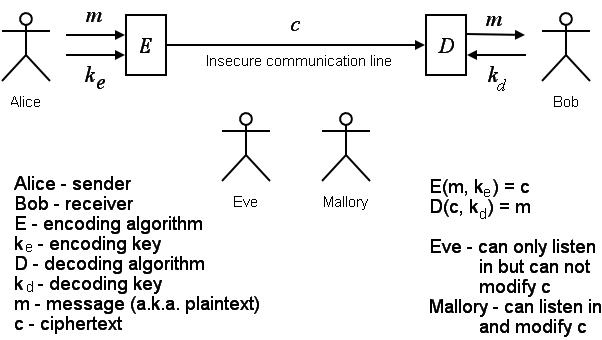
\includegraphics[width=8cm, height=5cm]{./pics/cryptosystem.png}};
        \begin{scope}[x={(image.south east)},y={(image.north west)}]
        %\draw[help lines,xstep=.1,ystep=.1] (0,0) grid (1,1);
        %\foreach \x in {0,1,...,9} { \node [anchor=north] at (\x/10,0) {0.\x}; }
        %\foreach \y in {0,1,...,9} { \node [anchor=east] at (0,\y/10) {0.\y}; }
        \draw[black, thin, rounded corners] (-0.1,0.0) rectangle (1.1,1.0);

    \end{scope}

  \end{tikzpicture}
  \end{center}
}

\frame
{
  \frametitle{What is cryptography?}

    \textit{``\textcolor{red}{Cryptography} is about constructing and analyzing protocols that prevent third parties or the public from reading private messages." \scriptsize{\rightline{- M. Bellare and P. Rogaway, Introduction to Modern Cryptography}}}

    \begin{center}
    \begin{tikzpicture}
    \node[anchor=south west,inner sep=0] (image) at (0,0) { 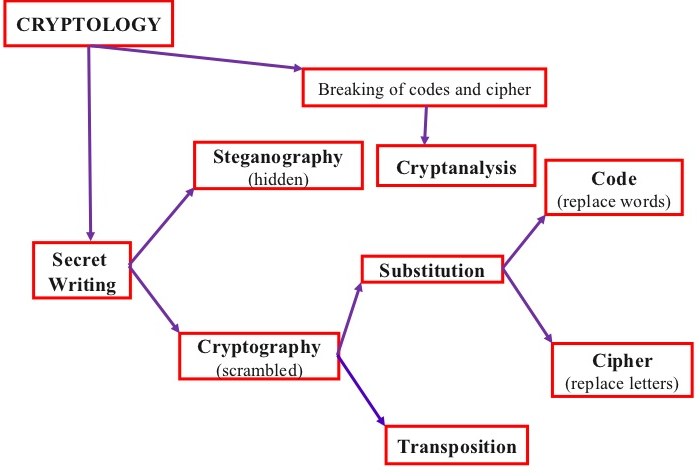
\includegraphics[width=10cm, height=6cm]{./pics/cryptography.png}};

    \begin{scope}[x={(image.south east)},y={(image.north west)}]
        %\draw[help lines,xstep=.1,ystep=.1] (0,0) grid (1,1);
        %\foreach \x in {0,1,...,9} { \node [anchor=north] at (\x/10,0) {0.\x}; }
        %\foreach \y in {0,1,...,9} { \node [anchor=east] at (0,\y/10) {0.\y}; }
        \draw[green, ultra thick, rounded corners] (0.24,0.18) rectangle (0.50,0.32);
    \end{scope}
    \end{tikzpicture}
    \end{center}

}

\frame
{
 \frametitle{Why we need cryptography in communications?}

 \begin{itemize}
 \setlength{\itemsep}{12pt}
 %\setlength{\parsep}{0pt}
 %\setlength{\parskip}{0pt}
 %\textcolor{red/blue/green/black/white/cyan/magenta/yellow}{text}
 \item \textcolor{red}{\underline{C}onfidentiality}: not just mean en/decryption, it imposes allow authorized people access privileged data.
 \item \textcolor{magenta}{\underline{I}ntegrity}: not just mean signature, it includes how to prove the originality and the tractability of the data.
 \item \textcolor{blue}{\underline{A}uthenticity}: User and device must be authenticated for services.
 \end{itemize}
}


\section{The ``key" problem in crypography}

\frame
{
\frametitle{The Kerckhoffs principle in cryptography}
\begin{columns}[c]
\column{.65\textwidth}
\begin{itemize}
\setlength{\itemsep}{12pt}
\item Do not rely on keeping an algorithm secret.
\item Publish an algorithm but keep the key secretly.
\item \textcolor{red}{Have some mathematical foundation for the belief that it will be hard to extract the key.}
\end{itemize}

\column{.35\textwidth}
\begin{figure}[htbp]
\centering
  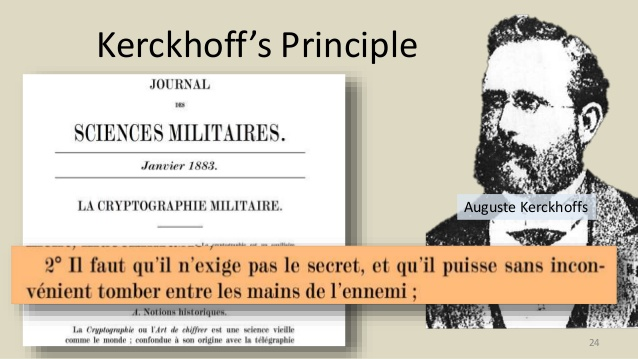
\includegraphics[width=4cm]{./pics/Kerckhoff.jpg}
\end{figure}

\end{columns}
}

\frame
{
\frametitle{Different key types in cryptosystems}
\begin{center}
\begin{tikzpicture}
    \node[anchor=south west,inner sep=0] (image) at (0,0) { 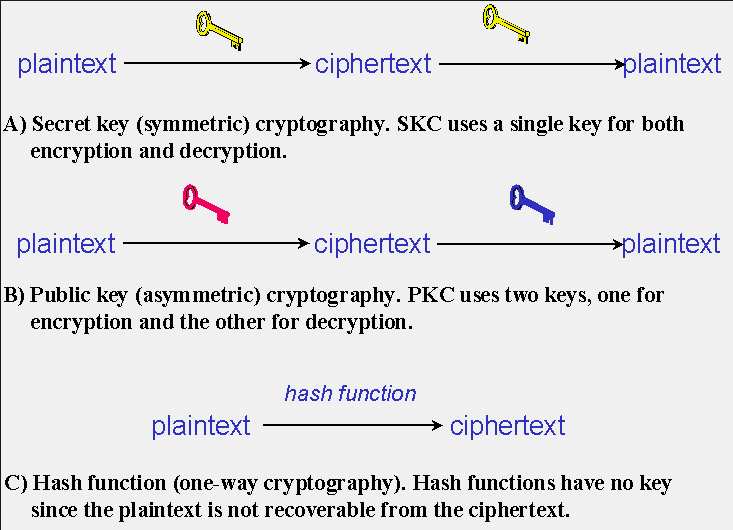
\includegraphics[width=8.5cm, height=5.5cm]{./pics/crypto_key_types.png}};

    \begin{scope}[x={(image.south east)},y={(image.north west)}]
        %\draw[help lines,xstep=.1,ystep=.1] (0,0) grid (1,1);
        %\foreach \x in {0,1,...,9} { \node [anchor=north] at (\x/10,0) {0.\x}; }
        %\foreach \y in {0,1,...,9} { \node [anchor=east] at (0,\y/10) {0.\y}; }
        \draw[black, thin, rounded corners] (0.0,-0.05) rectangle (1.0,1.05);
        \draw[red,line width=1pt](0.04,0.74)--(0.34,0.74);
        \draw[red,line width=1pt](0.04,0.42)--(0.35,0.42);
        \draw[red,line width=1pt](0.24,0.06)--(0.55,0.06);
        %\draw[line width=2pt,-latex](0,0)--(8,0);
    \end{scope}
\end{tikzpicture}
\end{center}
}



\frame
{
\frametitle{Threats of secret key in mobile applications}
\begin{itemize}
 \setlength{\itemsep}{12pt}
\item There are three types of threats in mobile applications.
\begin{itemize}
\setlength{\itemsep}{12pt}
\item Benign host, Malicious client (APPs)
\item Malicious host, Malicious client (Cloud service)
\item Benign host, Benign client (VPN)
\end{itemize}
\setlength{\itemsep}{12pt}
\item In most of mobile applications, hosts are assumed to be benign whilst client might be malicious or controlled by adversary.
\end{itemize}
}


\frame
{
\frametitle{Hardware-aided key protection}
In practice, many kinds of hardware are used for protecting secret key in practice.
\begin{columns}[c]
\column{.6\textwidth}
\begin{itemize}
\setlength{\itemsep}{12pt}
\item PC environment: TPMs, USB keys, Intel SGX.
\item Mobile environment: TEE, SE, MicroUSB/Bluetooth USB keys.
\end{itemize}
\column{.4\textwidth}
\begin{figure}[htbp]
\centering
  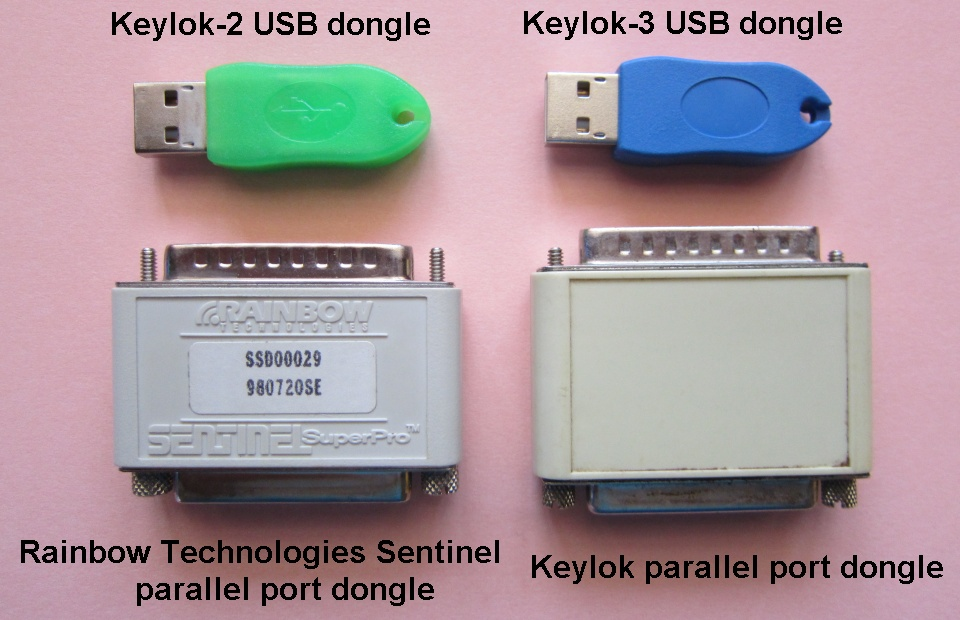
\includegraphics[width=4.8cm]{./pics/dongles.jpg}
\end{figure}
\end{columns}


\textcolor{red}{Problem:} Hardware-aided solutions can hardly be compatible in various mobile devices and their platforms.
}

\frame
{
\frametitle{``counter-examples" on the hardware interoperability}

\begin{figure}
\centering
\begin{minipage}[b]{0.3\textwidth}
\centering
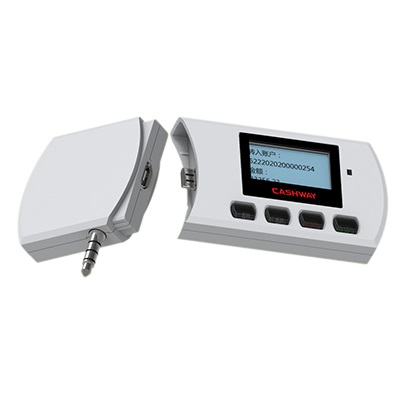
\includegraphics[width=3cm]{./pics/mickey.jpg}
%\parbox{.45\linewidth}{\centering\small a.aa}
\end{minipage}%
\hspace{0.04\textwidth}%
\begin{minipage}[b]{0.3\textwidth}
\centering
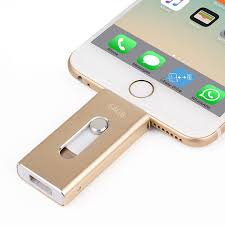
\includegraphics[width=3cm]{./pics/iphonekey.jpeg}
%\parbox{.45\linewidth}{\centering\small b.bb}
\end{minipage}\\[20pt]
\begin{minipage}[b]{0.3\textwidth}
\centering
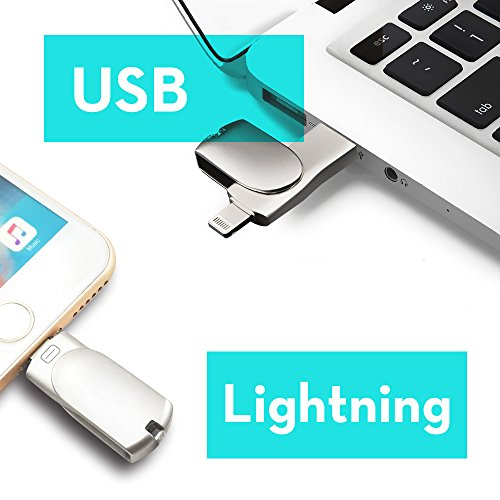
\includegraphics[width=2.7cm]{./pics/usb-lightning.jpg}
%\parbox{.45\linewidth}{\centering\small c.cc}
\end{minipage}
\begin{minipage}[b]{0.3\textwidth}
\centering
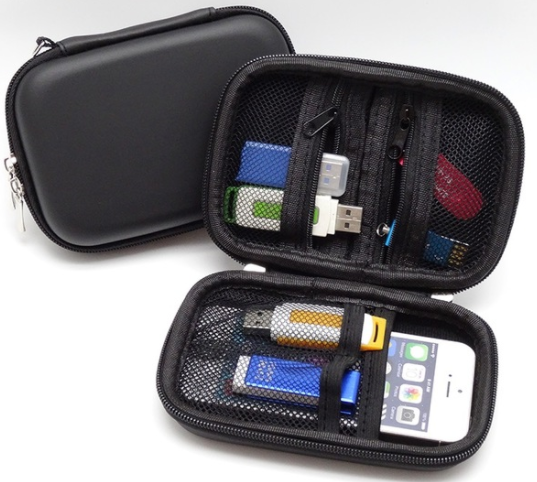
\includegraphics[width=3cm]{./pics/keyproblem.png}
%\parbox{.45\linewidth}{\centering\small c.cc}
\end{minipage}
\end{figure}
}

\frame
{
\frametitle{Threat in software solutions}
Although software solutions enjoy the interoperability and flexibility, the security problems rise.
\begin{itemize}
\setlength{\itemsep}{12pt}
\item Emulation
\item Run step-by-step in a debugger
\item Disassemble/decompile
\end{itemize}

\begin{figure}[htbp]
\centering
  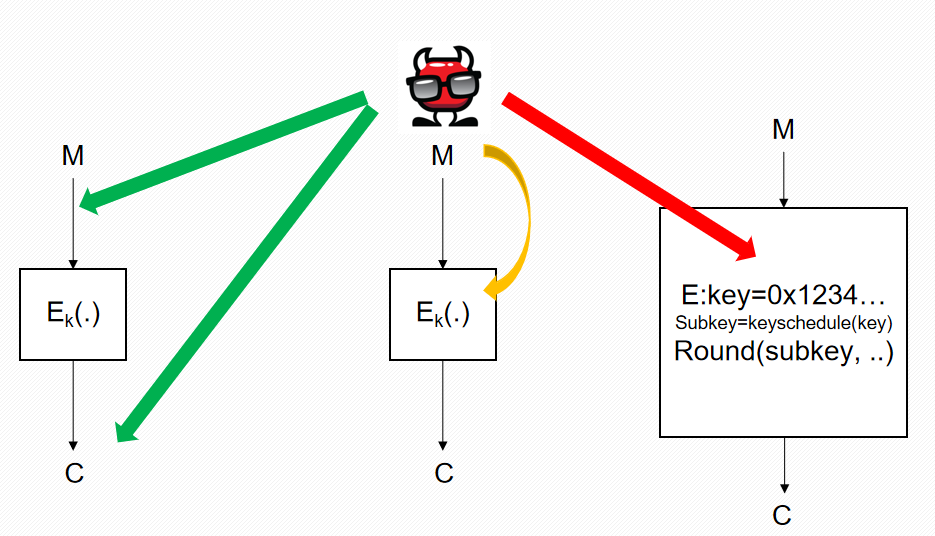
\includegraphics[width=8cm]{./pics/WBC_Model.png}
\end{figure}

}

\frame{
\frametitle{Black/White/Grey-box models}
\begin{block}{Black-box model}
\begin{itemize}
\item The adversary is able to know, (adaptively) choose inputs and obtain outputs.

\item Given the black-box implementation of the function, the adversary aims to \textcolor{red}{recover the secret values} or to \textcolor{orange}{misbehave the function}.
\end{itemize}
\end{block}

\begin{alertblock}{White-box model}
\begin{itemize}
\item The adversary can tamper, modify, manipulate all intermediate values and processes of the implementation of a secrecy system.
\item \alert{full knowledge} of the underlying cryptosystem \alert{except the secret values}.
\end{itemize}
\end{alertblock}

\begin{block}{Grey-box model}
According to the black/white-box models, a grey-box adversary is able to
\begin{itemize}
\item know, choose or adaptively choose inputs and outputs of the function;
\item tamper, modify, manipulate intermediate values with specific knowledge.

\end{itemize}
\end{block}
}

\frame{
\frametitle{An illustration of the black/white/grey-box models}
\begin{figure}[htbp]
\centering
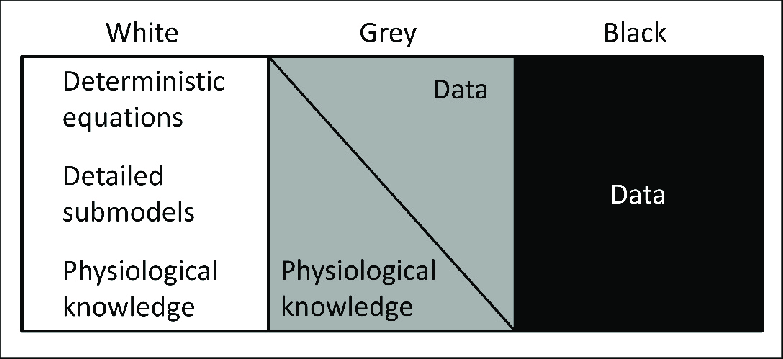
\includegraphics[width=9cm,height=4cm]{./pics/Illustration-of-the-concept-of-Black-White-Grey-box-modeling.png};
\end{figure}
}

\frame
{
\frametitle{Applications of black/grey-model-secure products}
\begin{columns}[c]
\column{.6\textwidth}
\begin{itemize}
\item A typical example is the maturing of USB keys
\item The various manufactories and vendors provide different solutions to make RSA/ECC onboard (which also deliberately design to resist grey-box attackers).
\item Eventually it works like a secure black box (and still evolving)
\end{itemize}
\column{.4\textwidth}
\begin{figure}[htbp]
\centering
  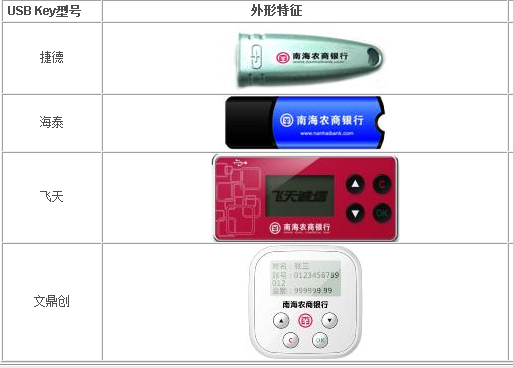
\includegraphics[width=4.8cm]{./pics/usbkey.png}
\end{figure}

\end{columns}

}

\frame
{
\frametitle{Software protection techniques}
\begin{itemize}
\item \textcolor[rgb]{1.00, 0.00, 0.00}{Reverse engineering attacks} - \textcolor[rgb]{0.00,1.00,0.00}{Code obfuscation}

\item \textcolor[rgb]{1.00, 0.00, 0.00}{Modification attacks} - \textcolor[rgb]{0.00,1.00,0.00}{Tamper resistance}

\item \textcolor[rgb]{1.00, 0.00, 0.00}{Program-based attacks} - \textcolor[rgb]{0.00,1.00,0.00}{Software diversity}

\item \textcolor[rgb]{1.00, 0.00, 0.00}{BORE (Break Once Run Everywhere) attacks} - \textcolor[rgb]{0.00,1.00,0.00}{Online/Offline registration verification}
\end{itemize}

In SAC 2002, Chow \textit{et al.} first proposed \textit{white-box cryptography} (WBC) which plays a pivotal role in cryptographic software protection.
}

\section{White-box crypogrpahy}

\frame{
\frametitle{The goal of modern cryptography}
\begin{alertblock}{}
The goal of modern cryptography is to design, analysis, and implement a cryptosystem which obtains \textcolor{red}{a mathematically acceptable security proofs on a certain model!}
\end{alertblock}
\begin{itemize}
\item From \textcolor{red}{theoretical} view:
\begin{itemize}
\item Ideal cipher/Random oracle model: Black-box analysis based on complexity
\item Indistinguishability/Indifferentiability model: Coin-tossing game
\item Key resilient/leakage model: Key-lossing assumption based provable security
\end{itemize}


\item From \textcolor{red}{heuristic} view:
\begin{itemize}
\item \textcolor{red}{Black/White/Grey-box models}
\end{itemize}
\end{itemize}

}

\frame
{
\frametitle{Why we need white-box cryptography?}
\begin{itemize}
\setlength{\itemsep}{12pt}
\item Although hardware-protected black/grey-box solutions are matured in the last decade, software solutions are still useful in many areas.

\item To the best of my knowledge, the white-box crypto (which includes symmetric/asymmetric-key cryptosystems) is pivotal for the following practical issues.
\begin{itemize}
\setlength{\itemsep}{12pt}
\item Hardware protection is costly (\textcolor{red}{price})
\item Hardware solution is incompatible (\textcolor{red}{interoperability})
\item Extreme system security protection (\textcolor{red}{key obfuscation})
\item Algorithm implementation flexibility and complexity (\textcolor{red}{Complex functionality requirements})
\end{itemize}
\end{itemize}

}

\frame
{
\frametitle{A typical white-box crypto in a nutshell}
\begin{figure}[htbp]
\centering
  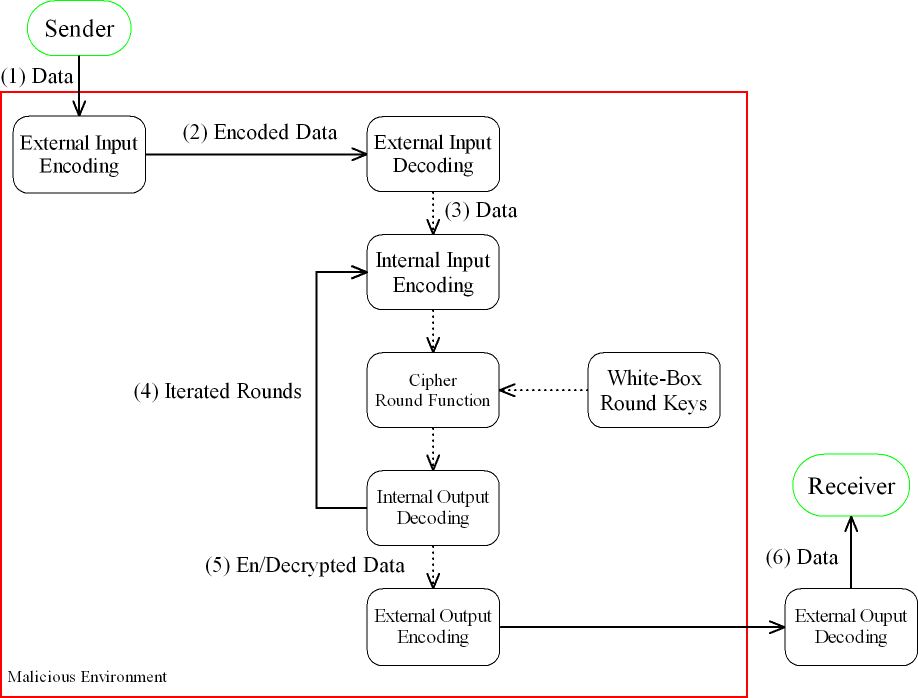
\includegraphics[width=10cm]{./pics/WBCrypto_Functional_Model.png}

\end{figure}

}

\frame
{
\frametitle{The pivotal role that WBC plays in mobile applications}
\begin{itemize}
\setlength{\itemsep}{12pt}
\item Mobile Payment: User authentication, transaction integrity.

\item Digital Rights Management: User authentication, Content anti-piracy.

\item Mobile OA (Office Automation): Digital signature, data protection.
\end{itemize}

}

\frame
{
\frametitle{WBC in mobile applications}
\begin{center}
\begin{tikzpicture}
    \node[anchor=south west,inner sep=0] (image) at (0,0) { 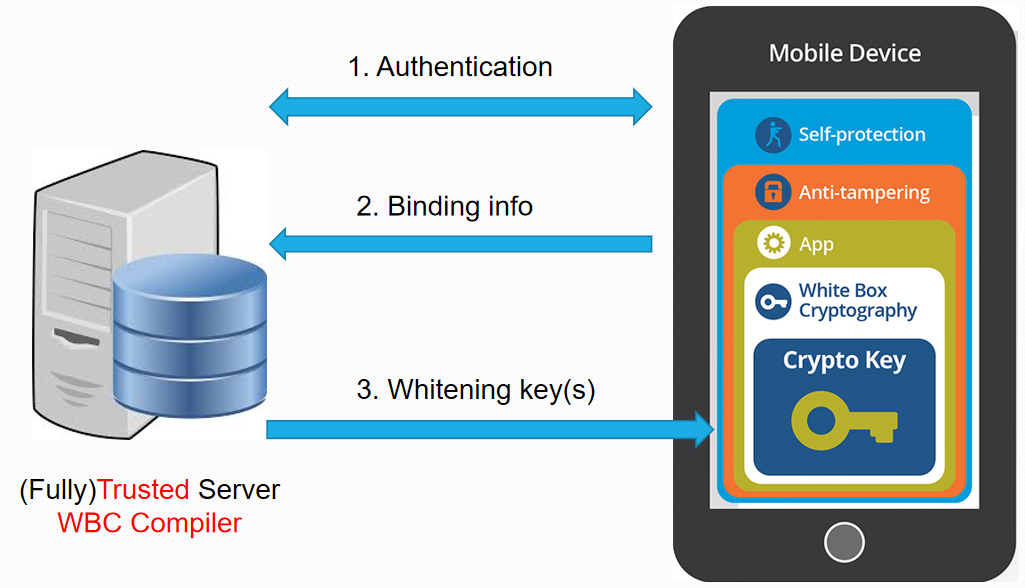
\includegraphics[width=10cm, height=6cm]{./pics/WBC_MobileApplication.png}};

    %\begin{scope}[x={(image.south east)},y={(image.north west)}]
        %\draw[help lines,xstep=.1,ystep=.1] (0,0) grid (1,1);
        %\foreach \x in {0,1,...,9} { \node [anchor=north] at (\x/10,0) {0.\x}; }
        %\foreach \y in {0,1,...,9} { \node [anchor=east] at (0,\y/10) {0.\y}; }
        %\draw[green, ultra thick, rounded corners] (0.24,0.18) rectangle (0.50,0.32);
    %\end{scope}
\end{tikzpicture}
\end{center}

}

\frame
{
\frametitle{Informal definitions of white-box crypto (in mobile applications)}
Informally I have the following concerns about white-box crypto:
\begin{itemize}
\setlength{\itemsep}{12pt}
\item From the view of crypto key security, it implies
\begin{itemize}
\setlength{\itemsep}{12pt}
\item secret key protection: adversary cannot extract secret key from software (no matter whether running or not).

\item key distribution mechanism: only designated user/server can generate the white-box version secret key (quite close to public-key crypto, but not exactly the same).

\end{itemize}
\end{itemize}
}

\frame
{
\frametitle{Informal definitions of white-box crypto (in mobile applications)}
\begin{itemize}
\setlength{\itemsep}{12pt}
\item From the view of software developer, it implies
\begin{itemize}
\setlength{\itemsep}{12pt}
\item Cryptographic obfuscation: the algorithm is public, but only the secret key is obfuscated.

\item Code/space/time hardness: the time/memory/space complexities will increased (heavily).

\item Function abstraction: After white-box implementation, a function's inner functionality is no longer publicly verifiable.
\end{itemize}
\end{itemize}

}

\frame
{
\frametitle{Differences between software obfuscation and white-box cryptography}
Software obfuscation and white-box crypto can operate together to achieve concrete security, while they have different purposes:
\begin{itemize}
\setlength{\itemsep}{12pt}
\item Software obfuscation does not look for theoretically secure levels of white-box crypto, it should be feasible for practice

\item White-box crypto must be secure either in theory or computational complexity

\item Software obfuscation merely seeks to increase the reverse-engineering costs in a sufficiently discouraging manner for adversary
\end{itemize}

}

\frame
{
\frametitle{White-box cryptography working range}
\begin{itemize}
\setlength{\itemsep}{12pt}
\item To resist adversary, a software should be secure against:
\begin{itemize}
\setlength{\itemsep}{12pt}
\item Static analysis: from binary code to extract information

\item Dynamic analysis: from memory to extract information

\item Code lifting: change the execution order/function, which breaks the integrity of software
\end{itemize}

\item For white-box crypto, the priority of security goals are listed as follows.
\begin{itemize}
\setlength{\itemsep}{12pt}
\item Functionality is executed as designed.

\item Secret key (or its equivalence) cannot leaked.

\item Application/device-binding property.
\end{itemize}

\end{itemize}

}


\section{The State-of-the-art of white-box cryptography}

\frame
{
\frametitle{The State-of-the-art of white-box cryptography}
\begin{itemize}
\setlength{\itemsep}{12pt}
\item Security notions and definitions.

\item WBC proposals and implementations.

\item WBC cryptanalsis techniques.

\item WBC applications.

\end{itemize}
}

%\frame
%{
%\frametitle{Basic security definitions for white-box crypto (1)}
%\begin{itemize}
%\item In SAC 2002, the security notions have been defined by Chow \textit{et al.}. First the key recovery problem is informally defined by \textcolor{red}{the weak white-box security}.
%\end{itemize}
%
%
%\begin{center}
%\begin{tikzpicture}
%    \node[anchor=south west,inner sep=0] (image) at (0,0) { 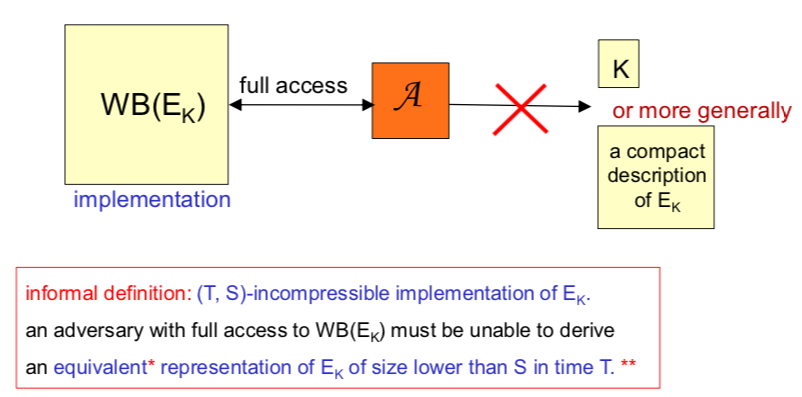
\includegraphics[width=8cm, height=4cm]{./pics/weak_white_box_security.png}};
%
%    \begin{scope}[x={(image.south east)},y={(image.north west)}]
%        %\draw[help lines,xstep=.1,ystep=.1] (0,0) grid (1,1);
%        %\foreach \x in {0,1,...,9} { \node [anchor=north] at (\x/10,0) {0.\x}; }
%        %\foreach \y in {0,1,...,9} { \node [anchor=east] at (0,\y/10) {0.\y}; }
%        \draw[red, thin, rounded corners] (0.85,0.7) circle (1.2cm);
%    \end{scope}
%\end{tikzpicture}
%\end{center}
%}
%
%\frame
%{
%\frametitle{Basic security definitions for white-box crypto(2)}
%\begin{itemize}
%\item For more general security, \textcolor{red}{the strong white-box security} has been defined by Biryukov \textit{et al.} at ASIACRYPT 2014.
%\end{itemize}
%
%\begin{center}
%\begin{tikzpicture}
%    \node[anchor=south west,inner sep=0] (image) at (0,0) { 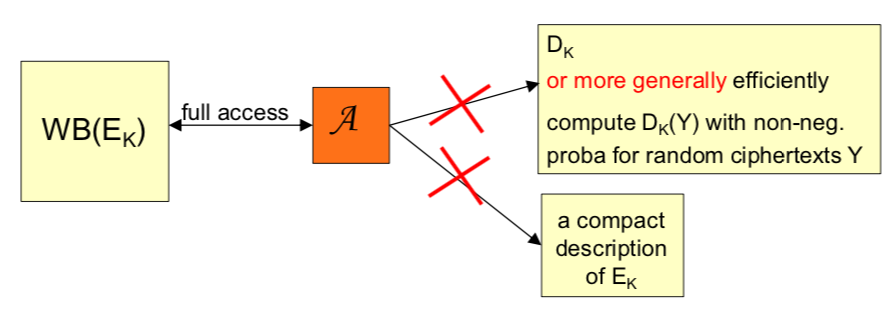
\includegraphics[width=10cm, height=4cm]{./pics/strong_white_box_security.png}};
%
%    %\begin{scope}[x={(image.south east)},y={(image.north west)}]
%        %\draw[help lines,xstep=.1,ystep=.1] (0,0) grid (1,1);
%        %\foreach \x in {0,1,...,9} { \node [anchor=north] at (\x/10,0) {0.\x}; }
%        %\foreach \y in {0,1,...,9} { \node [anchor=east] at (0,\y/10) {0.\y}; }
%        %\draw[green, ultra thick, rounded corners] (0.24,0.18) rectangle (0.50,0.32);
%    %\end{scope}
%\end{tikzpicture}
%\end{center}
%}
%
%\frame
%{
%\frametitle{Provable security of WBC}
%
%\begin{itemize}
%\item Saxena \textit{et al.} proposed security notions and a provable secure case ECC pairing for WBC at ISC 2009.
%
%\item Delerablee \textit{et al.} extended Saxena \textit{et al.}'s work and proposed an RSA-based WBC at SAC 2013.
%
%\item Biyukov \textit{et al.} proposed weak/strong white-box security notions at ASIACRYPT 2014.
%
%\item Foque \textit{et al.} improved the notions with WhiteBlock at ASIACRYPT 2016.
%
%\item Biyukov and Perrin. proposed symmetrically/asymmetrically hard security model at Crypto 2017.
%
%\item Bock \textit{et al.} proposed Indistinguishability for White-Box Hardware/Application Binding at CHES 2020.
%
%\end{itemize}
%
%}
%
%\frame
%{
%\frametitle{WBC Implementations of DES/AES/SM4 (All broken!)}
%\begin{itemize}
%\item Chow \textit{et al.} Tbox-based WBDES/AES, 2002
%\item Bringer. Isomorphism of Polynomials, WBAES, 2006
%\item Xiao and Lai. 16-bit Tbox WBAES, 2009
%\item Xiao and Lai. Affine-function WBSM4, 2009
%\item Karroumi \textit{et al.} Dual-cipher WBAES, 2011
%\item Baek \textit{et al.} Larger Tbox WBAES, 2016
%\item Lee \textit{et al.} Masked WBAES, 2018
%\item Xu \textit{et al.} Obfuscated round boundaries WBAES/SM4, 2018
%\item Lee and Kim. Table redundancy WBAES, 2019
%\end{itemize}
%}
%
%\frame
%{
%\frametitle{Dedicated WBC Proposals}
%\begin{itemize}
%\item Biyukov \textit{et al.} ASASA structure, 2014
%\item Bogdanov and Isobe. SPACE, 2015
%\item Bogdanov and Isobe. SPNbox, 2016
%\item Cho and Dinur. WEM, 2017
%\item Zhou \textit{et al.} Lightweight WBC, 2018
%\item Lv \textit{et al.} WB-KMAC, 2019
%\item Shi \textit{et al.} SDSRS, 2020
%\item Kwon \textit{et al.} FPL, 2020
%\end{itemize}
%}
%
%\frame
%{
%\frametitle{Algebraic cryptanalysis techniques for WBC}
%\begin{itemize}
%\item BGE attack on WB-AES
%\begin{itemize}
%\item Billet et al. 2004
%\end{itemize}
%
%\item Generic attack on SPN structure WBC
%\begin{itemize}
%\item Michiels et al. 2008
%\end{itemize}
%
%\item Attack on the variants
%\begin{itemize}
%\item De Mulder et al. 2010
%\item De Mulder et al. 2012
%\item Lepoint et al. 2013
%\item Derbez 2017
%\end{itemize}
%\end{itemize}
%}
%
%\frame
%{
%\frametitle{Algebraic cryptanalysis on WBAES/SM4}
%\begin{figure}[htbp]
%\centering
%  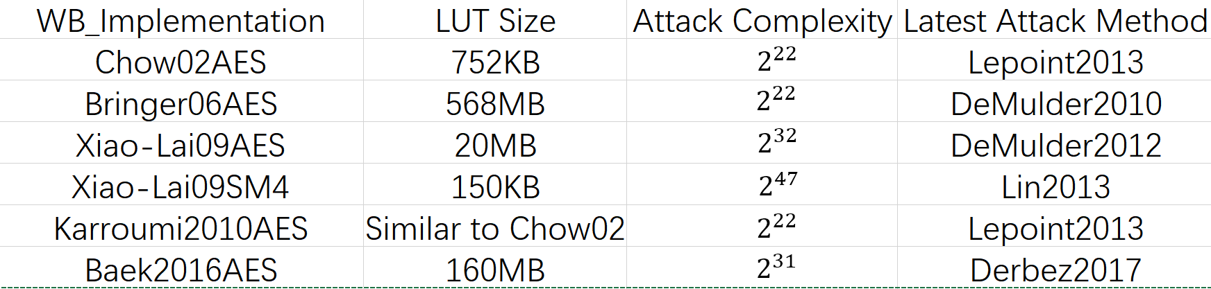
\includegraphics[width=10cm]{./pics/WBCCryptanlysis.png}
%\end{figure}
%}
%
%\frame
%{
%\frametitle{Side-channel techniques for WBC}
%
%\begin{itemize}
%\item Bos \textit{et al.} Differential computation/fault analysis (DCA/DFA), 2016
%
%\item Goubin \textit{et al.} Linear Decoding Analysis, 2018
%
%\item Bock \textit{et al.} Dynamic Binary Instrumentation (DBI), 2019
%
%\item Zeyad \textit{et al.} Statistical Bucketing Attack (SBA), 2019
%
%\item Bogdanov \textit{et al.} High-order DCA, 2019
%
%\item Rivain and Wang. Improved DCA, 2019
%
%\item Amadori \textit{et al.} BGE+DFA, breaks 8-bit external output encoding, 2019
%
%\end{itemize}
%
%}
%
%\frame
%{
%\frametitle{WBC applications}
%
%\begin{itemize}
%\item Academic proposals
%\begin{itemize}
%\item Software tamper resistance:
%\begin{itemize}
%\item Michiels and Gorissen, DRM 2007;
%\item Lin \textit{et al.}, iSCI 2019.
%\end{itemize}
%
%\item Digital rights management: Liu and Hu, ePrint 2017.
%
%\item IoT application: Shi \textit{et al.}, 2020.
%
%\end{itemize}
%
%\item Industrial products
%\begin{itemize}
%\item Irdeto, cloakware.
%\item Intertrust, whiteCryption.
%\item Denuvo, game anti-piracy.
%\end{itemize}
%\end{itemize}
%
%}

\section{Conclusion}

\frame
{
\frametitle{Conclusion}

\begin{itemize}
\setlength{\itemsep}{12pt}
\item White-box cryptography is practical for protecting mobile applications.

\item Software obfuscation and white-box cryptography are different fruits on the same tree.

\item Mobile applications have various requirements on white-box crypto.

\end{itemize}

}

\frame
{
\begin{center}
\textbf{Thanks for your attentions!}

\end{center}

\begin{center}
\begin{tikzpicture}
    \node[anchor=south west,inner sep=0] (image) at (0,0) { 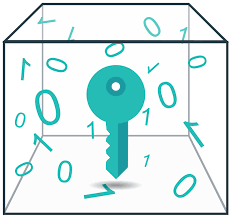
\includegraphics[width=4cm, height=4cm]{./pics/WBC_BG.png}};

    %\begin{scope}[x={(image.south east)},y={(image.north west)}]
        %\draw[help lines,xstep=.1,ystep=.1] (0,0) grid (1,1);
        %\foreach \x in {0,1,...,9} { \node [anchor=north] at (\x/10,0) {0.\x}; }
        %\foreach \y in {0,1,...,9} { \node [anchor=east] at (0,\y/10) {0.\y}; }
        %\draw[green, ultra thick, rounded corners] (0.24,0.18) rectangle (0.50,0.32);
    %\end{scope}
\end{tikzpicture}

\end{center}
}

\end{document}
